% !TeX root = ../../main.tex
\section{Smart Device}\label{section:smart-device}

The \enquote{Smart Device} is a part of the \ac{UBII} front end. Because it is web-based, only data which is available through the \textbf{Web \acp{API}} can be obtained. Since it was not designed for a specific use case, it is thought as general purpose or testing device. Only touch positions, touch events, orientation and acceleration is sent to different topics using the \textbf{\ac{UBII} Client}. For more specific scenarios, the smart device can not be used and a custom interface has to be implemented. For the experiments in this thesis though, the smart device client was sufficient, after implementing some improvements.

The data which is published, is also displayed on the screen for debugging purposes. It is possible to set the view in full screen mode, to prevent unintentional interactions with control elements of the web browser or the operating system. Since the reference system for the orientation is fixed to the earth~\cite[Chapter~4.1]{DevicesandSensorsWorkingGroup.2019}, a calibration system was implemented. With the press of the \enquote{Calibrate} button, the device is calibrated to the new orientation.


\subsection{ORientation}\label{subsection:orientation}

The orientation is provided by the \textbf{Web API} through the \lstinline{DeviceOrientation} event. The orientation is desribed by three values named \lstinline{alpha}, \lstinline{beta} and \lstinline{gamma}, as seen in figure~\ref{fig:webapi-device-orientation}. 
% TODO: values are smoothed and interpolated.... cite?
While \lstinline{alpha} returns values from $0$ to $360$ in euler angles, \lstinline{beta} only returns $bla$ and \lstinline{gamma} $bla$~\cite{DevicesandSensorsWorkingGroup.2019}.
% <- todo cite chapter 
This limitation entails that no full orientation tracking is possible with this event. 

\begin{figure}[htpb]
  \centering
  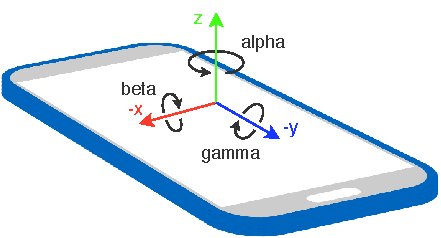
\includegraphics[height=5cm]{figures/webapi_device_orientation.pdf}
  \caption[Device Orientation]{The specification of the orientation values visualized. The $x$ and $y$ axes are inverted for the sake of clarity.}\label{fig:webapi-device-orientation}
\end{figure}

The \textbf{Web API} also provides the \lstinline{MotionEvent}, which returns multiple vectors, one beeing the acceleration with the gravity (\lstinline{accelerationWithGravity}). Since the gravity vector always points down, this vector can be used as a reference vector. Together with the values from the \lstinline{DeviceOrientation} event, the full orientation can be derived. The resulting orientation, then has to be smoothed out, because the accerleration vector uses the raw \ac{IMU} output. 

The data from the \lstinline{DeviceOrientation} already provides all three euler angles and is smoothed. Implementing the same for the data from the \lstinline{MotionEvent}, would be outside of the scope of this thesis. Because of this consideration, the smart device uses the \lstinline{DeviceOrientation} event data.

\subsection{Architecture}\label{subsection:architecture}

The touch position, is normalized to numbers from $0$ to $1$. This removes the influence from the display resolution and size. Touch events for start and stop touching are sent on a differen topic. 
% acceleration is also sent?

The smart device is registered as a device in the \ac{UBII} network and can be seen in figure % todo: ref to fig

% show listing of device smart device register()



